\chapter{Analyse}

I dette kapitel vil vi gennemgå kravspecifikation til programmet, samt optegne og forklare forskellige modeller.


\section{Kravspecifikation}
\label{sec:requirements}

\begin{enumerate}
    \item Spillet spilles af 2 spillere.
    \item Spillerne starter med en pengebeholdning på 1000kr og vinder, når pengebeholdning er 3000kr.
    \item Spilleren og hans pengebeholdning skal kunne bruges i andre spil.
    \item Spillet skal indeholde 12 felter, svarende til summen af terningerne (2-12), der vil altså kun være 11 brugbare felter, da man ikke kan slå 1 med to terninger.
    \item Hvert felt skal påvirke spillerens pengebeholdning forskelligt, og have en udskrift om hvilket felt han ramte.
    \item Hvis en spiller slår summen 10, tildeles denne spiller en ekstra tur.
    \item Det skal være let at skifte til andre terninger.
    \item Det skal kunne oversættes til andre sprog.
    \item Spillet skal kunne spilles uden bemærkelsesværdige forsinkelser.
    \item Det skal være muligt at kunne arbejde videre på systemet samt følge hvordan udviklingen er foregået.
    \\
\end{enumerate}

\pagebreak

\subsection{FURPS+ \& MoSCoW}

\subsubsection{FURPS+}
FURPS+ er en metode til at kategorisere / klassificere krav. \autocite{lecture:02313_lec2}
\\
Det plus vi ser til sidst i FURPS+ vises på mange forskellige måder, og er ikke altid det samme i alle sammenhænge.

\begin{figure*}[ht]{
    \centering
\begin{tabular}{|c | p{0,05cm} p{2,8cm} |p{10,5cm}|}
       \hline
       \textbf{F}   &   Functionality   &&
       Egenskaber, ydeevne, sikkerhed                   \\
       \hline

       \textbf{U}   &   Usability       &&
       Menneskelige faktorer, hjælp, dokumentation      \\
       \hline

       \textbf{R}   &   Reliability     &&
       Fejlfrekvens, fejlretning, forudsigelighed       \\
       \hline

       \textbf{P}   &   Performance     &&
       Svartider, nøjagtighed, ydeevne, ressourceforbrug                                                      \\
       \hline

       \textbf{S}   &   Supportability  &&
       Anvendelighed, tilpasningsevne, vedligeholdbarhed                                                      \\
       \hline

       \textbf{+}   &                   &&              \\

       &&   Implementation: &   Ressourcebegrænsninger, sprog og værktøjer, hardware                     \\

       &&   Interface:      &   Begrænsninger forårsaget af kommunikation med eksterne systemer              \\

       &&   Operations:     &   Systemstyring i dets operationelle ramme                              \\

       &&   Packaging:      &   F.eks. en fysisk boks   \\

       &&    Legal:         &   F.eks. licenser       \\
       \hline
\end{tabular}}
\end{figure*}

\noindent På denne måde kan vi så klassificere de enkelte krav:
\\\\\textbf{Functionality:}
\\ 2. Spillerne starter med en pengebeholdning på 1000kr og vinder, når pengebeholdning er 3000kr.
\\ 3. Spilleren og hans pengebeholdning skal kunne bruges i andre spil.
\\\\\textbf{Usability:}
\\1. Spillet spilles af 2 spillere.
\\ 5. Hvert felt skal påvirke spillerens pengebeholdning forskelligt, og have en udskrift om hvilket felt han ramte.
\\ 6. Hvis en spiller slår summen 10, tildeles denne spiller en ekstra tur.
\\\\\textbf{Performance:}
\\9. Spillet skal kunne spilles uden bemærkelsesværdige forsinkelser
\\\\\textbf{Supportability:}
\\ 3. Spilleren og hans pengebeholdning skal kunne bruges i andre spil.
\\ 7. Det let at skifte til andre terninger.
\\ 8. Spillet skal kunne let oversættes til andre sprog
\\ 10. Det skal være muligt at kunne arbejde videre på systemet samt følge hvordan udviklingen er foregået.
\\\\\textbf{(+) - Implementation:}
\\ 8. Spillet let oversættes til andre sprog
\\\\\\\\\textbf{(+) - Interface:}
\\ 4. Spillet skal indeholde 12 felter, svarende til summen af terningerne (2-12), der vil altså kun være 11 brugbare felter, da man ikke kan slå 1 med to terninger.

\subsubsection{MoSCoW}
MoSCoW, er et værktøj som kan bruges til at prioitere krav. \\\\
\begin{tabular}{lll}
    \textbf{Mo} &   
    "Must have"                 &
    De mest vitale krav, vi ikke kan undgå. \\

    \textbf{S}  &   
    "Should have"               & 
    Vigtige krav, som ikke er vitale. \\

    \textbf{Co} &   
    "Could have"                & 
    The 'nice-to-haves' \\

    \textbf{W}  &   
    "Won’t have (this time)"    & 
    Things that provide little to no value you can give up on \\
    
\end{tabular}

\begin{center}
    \begin{tabular}{ | l | p{13cm} |}
    \hline
    Must have & Spillerne skal have en pengebeholdning, der kan påvirkes både negativt og positivt.

    Spillet skal indeholde 11 brugbare felter svarende til summen af terningeslaget, hvert af disse felter skal påvirke spillernes pengebeholdning.

    Hvis en spiller slår summen 10, skal denne spiller have en ekstra tur.

    Spillet skal kunne spilles uden bemærkelsesværdige forsinkelser. En kort forklarende tekst til hvert felt. \\
    
    \hline
    Should have & Det skal være let at skifte terninger.

    Spillet skal kunne oversættes til andre sprog.

    Det skal være muligt at arbejde videre på systemet, og følge udviklingen af systemet. \\
    \hline
    Could have & En GUI til at vise felterne, samt til at vise terningens slag, spillers sum. \\
    \hline
    Won't have &  \\
    \hline
    \end{tabular}
\end{center}

\noindent
Vi har valgt ikke at have noget i won't have, da vi ummidelbart skal designe et færdiglavet program. Der er selvfølgelig plads til viderudvikling, hvilket ville ligge under won't have. Won't have kunne bruges til nogle features man ikke kan nå at få implementeret denne gang, men nogle man vil få implementeret fremtidigt.


\section{Interessentanalyse}
\begin{center}
    \begin{tabular}{ | l | p{13cm} |}
    \hline
    \textbf{Interresent} & \textbf{Interesse / Mål} \\ \hline
    Spiller/-e & Kunne styre et system, der styrer et spil mellem to personer, 
    hvor i der kastes med et raflebæger med to terninger i, og ser resultatet af dette slag med det samme, herefter skal summen af dette slag fortælle, hvilket felt spilleren landte på.\\ \hline
    \hline
    \end{tabular}
\end{center}

\pagebreak

\section{Use cases}

Følgende er en liste over use cases samt deres beskrivelser i en brief udgave.

\footnote{Use case modellen i tabel 3.1 er en revideret udgave af use case modellen fra CDIO 1 da vi har at gøre med en magen til konfiguration.}

\begin{table}[H]
    \begin{center}
        \begin{tabular}{ | p{15cm} |}
            \hline
            \textbf{Use case:} PlayGame \\ \hline
            \textbf{ID:} UC1 \\ \hline
            \textbf{Brief description} Spiller/-e skal kunne spille spil/Game (starte spillet) og slå med to terninger     \\ \hline
            \textbf{Primary actors:} Spiller/-e \\ \hline
            \textbf{Secondary actors:} Ingen. \\ \hline
            \textbf{Preconditions:} Ingen.     \\ \hline
            \textbf{Main flow:}
            \begin{enumerate}
                \item \textbf{Spiller 1 og spiller 2 tildeles 1000 i pengebeholdning}
                \item \textbf{Spiller 1 slår med to terninger, lander på et felt mellem 2-12 og bliver udefra det tildelt en opdateret pengebeholdning}
                \item \textbf{Spiller 2 slår med to terninger, lander på et felt mellem 2-12 og bliver udefra det tildelt en opdateret pengebeholdning}
                \item \textbf{Opnås 3000 i pengebeholdning, stoppes spillet} 
            \end{enumerate} \\ \hline
            \textbf{Postconditions:} Ingen.\\ \hline
            \textbf{Alternative flow:}
            \\- Ekstra ture gives ved, lande på feltet 'The Warewall (werewolf-wall)' \\ \hline
            \hline
        \end{tabular}
        \caption{Use case 1}
        \label{usecase:1}
    \end{center}
\end{table}

\pagebreak

\subsection{Use case diagram}

Til overblik over use cases er lavet en use case diagram.
Der er i dette tilfælde kun en use case, men vi har alligevel valgt at vise dette i figur \ref{fig:use_case_diagram}.\\

\begin{figure}[H]
    \begin{center}
        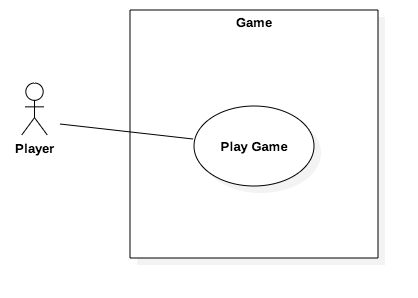
\includegraphics[width=15cm]{graphics/Use_Case_Diagram.png}
        \caption{Use case diagram}
        \label{fig:use_case_diagram}
    \end{center}
\end{figure}

\noindent Vi har i dette projekt én aktør i form a spilleren.
Denne aktør har kun en mulighed, og det er at spille spillet.
Der er derfor kun denne ene use case visualiseret.

\pagebreak

\section{Domænemodel}

Der er til projektet udarbejdet en domænemodel for at klarlægge projektets domæne.
Det ses her (figur \ref{fig:domaenemodel}), at spillet består af forskellige elementer som hver har deres forbindelse.
Hele domænet er omfattet af et spil (Game) som består af sprog (Language), terninger (Dice), spillere (Player) og en pengebeholdning (Stash).\\


\begin{figure}[H]
    \begin{center}
        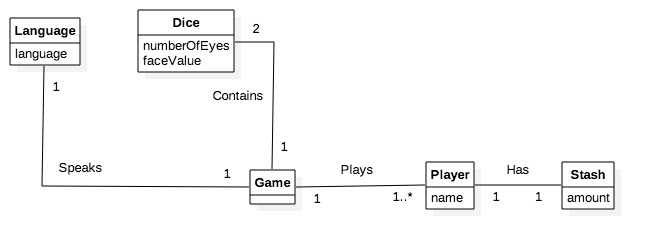
\includegraphics[width=15cm]{graphics/Domainmodel.png}
        \caption{Domænemodel over spillet}
        \label{fig:domaenemodel}
    \end{center}
\end{figure}